\documentclass[11pt,a4paper]{report}
\usepackage[textwidth=37em,vmargin=30mm]{geometry}
\usepackage{calc,xunicode,amsmath,amssymb,paralist,enumitem,tabu,booktabs,datetime2,xeCJK,xeCJKfntef,listings}
\usepackage{tocloft,fancyhdr,tcolorbox,xcolor,graphicx,eso-pic,xltxtra,xelatexemoji}

\newcommand{\envyear}[0]{2025}
\newcommand{\envdatestr}[0]{2025-08-10}
\newcommand{\envfinaldir}[0]{webdb/2025/20250810/final}

\usepackage[hidelinks]{hyperref}
\hypersetup{
    colorlinks=false,
    pdfpagemode=FullScreen,
    pdftitle={Web Digest - \envdatestr}
}

\setlength{\cftbeforechapskip}{10pt}
\renewcommand{\cftchapfont}{\rmfamily\bfseries\large\raggedright}
\setlength{\cftbeforesecskip}{2pt}
\renewcommand{\cftsecfont}{\sffamily\small\raggedright}

\setdefaultleftmargin{2em}{2em}{1em}{1em}{1em}{1em}

\usepackage{xeCJK,xeCJKfntef}
\xeCJKsetup{PunctStyle=plain,RubberPunctSkip=false,CJKglue=\strut\hskip 0pt plus 0.1em minus 0.05em,CJKecglue=\strut\hskip 0.22em plus 0.2em}
\XeTeXlinebreaklocale "zh"
\XeTeXlinebreakskip = 0pt


\setmainfont{Brygada 1918}
\setromanfont{Brygada 1918}
\setsansfont{IBM Plex Sans}
\setmonofont{JetBrains Mono NL}
\setCJKmainfont{Noto Serif CJK SC}
\setCJKromanfont{Noto Serif CJK SC}
\setCJKsansfont{Noto Sans CJK SC}
\setCJKmonofont{Noto Sans CJK SC}

\setlength{\parindent}{0pt}
\setlength{\parskip}{8pt}
\linespread{1.15}

\lstset{
	basicstyle=\ttfamily\footnotesize,
	numbersep=5pt,
	backgroundcolor=\color{black!5},
	showspaces=false,
	showstringspaces=false,
	showtabs=false,
	tabsize=2,
	captionpos=b,
	breaklines=true,
	breakatwhitespace=true,
	breakautoindent=true,
	linewidth=\textwidth
}






\newcommand{\coverpic}[2]{
    % argv: itemurl, authorname
    Cover photo by #2~~(\href{#1}{#1})
}
\newcommand{\makeheader}[0]{
    \begin{titlepage}
        % \newgeometry{hmargin=15mm,tmargin=21mm,bmargin=12mm}
        \begin{center}
            
            \rmfamily\scshape
            \fontspec{BaskervilleF}
            \fontspec{Old Standard}
            \fontsize{59pt}{70pt}\selectfont
            WEB\hfill DIGEST
            
            \vfill
            % \vskip 30pt
            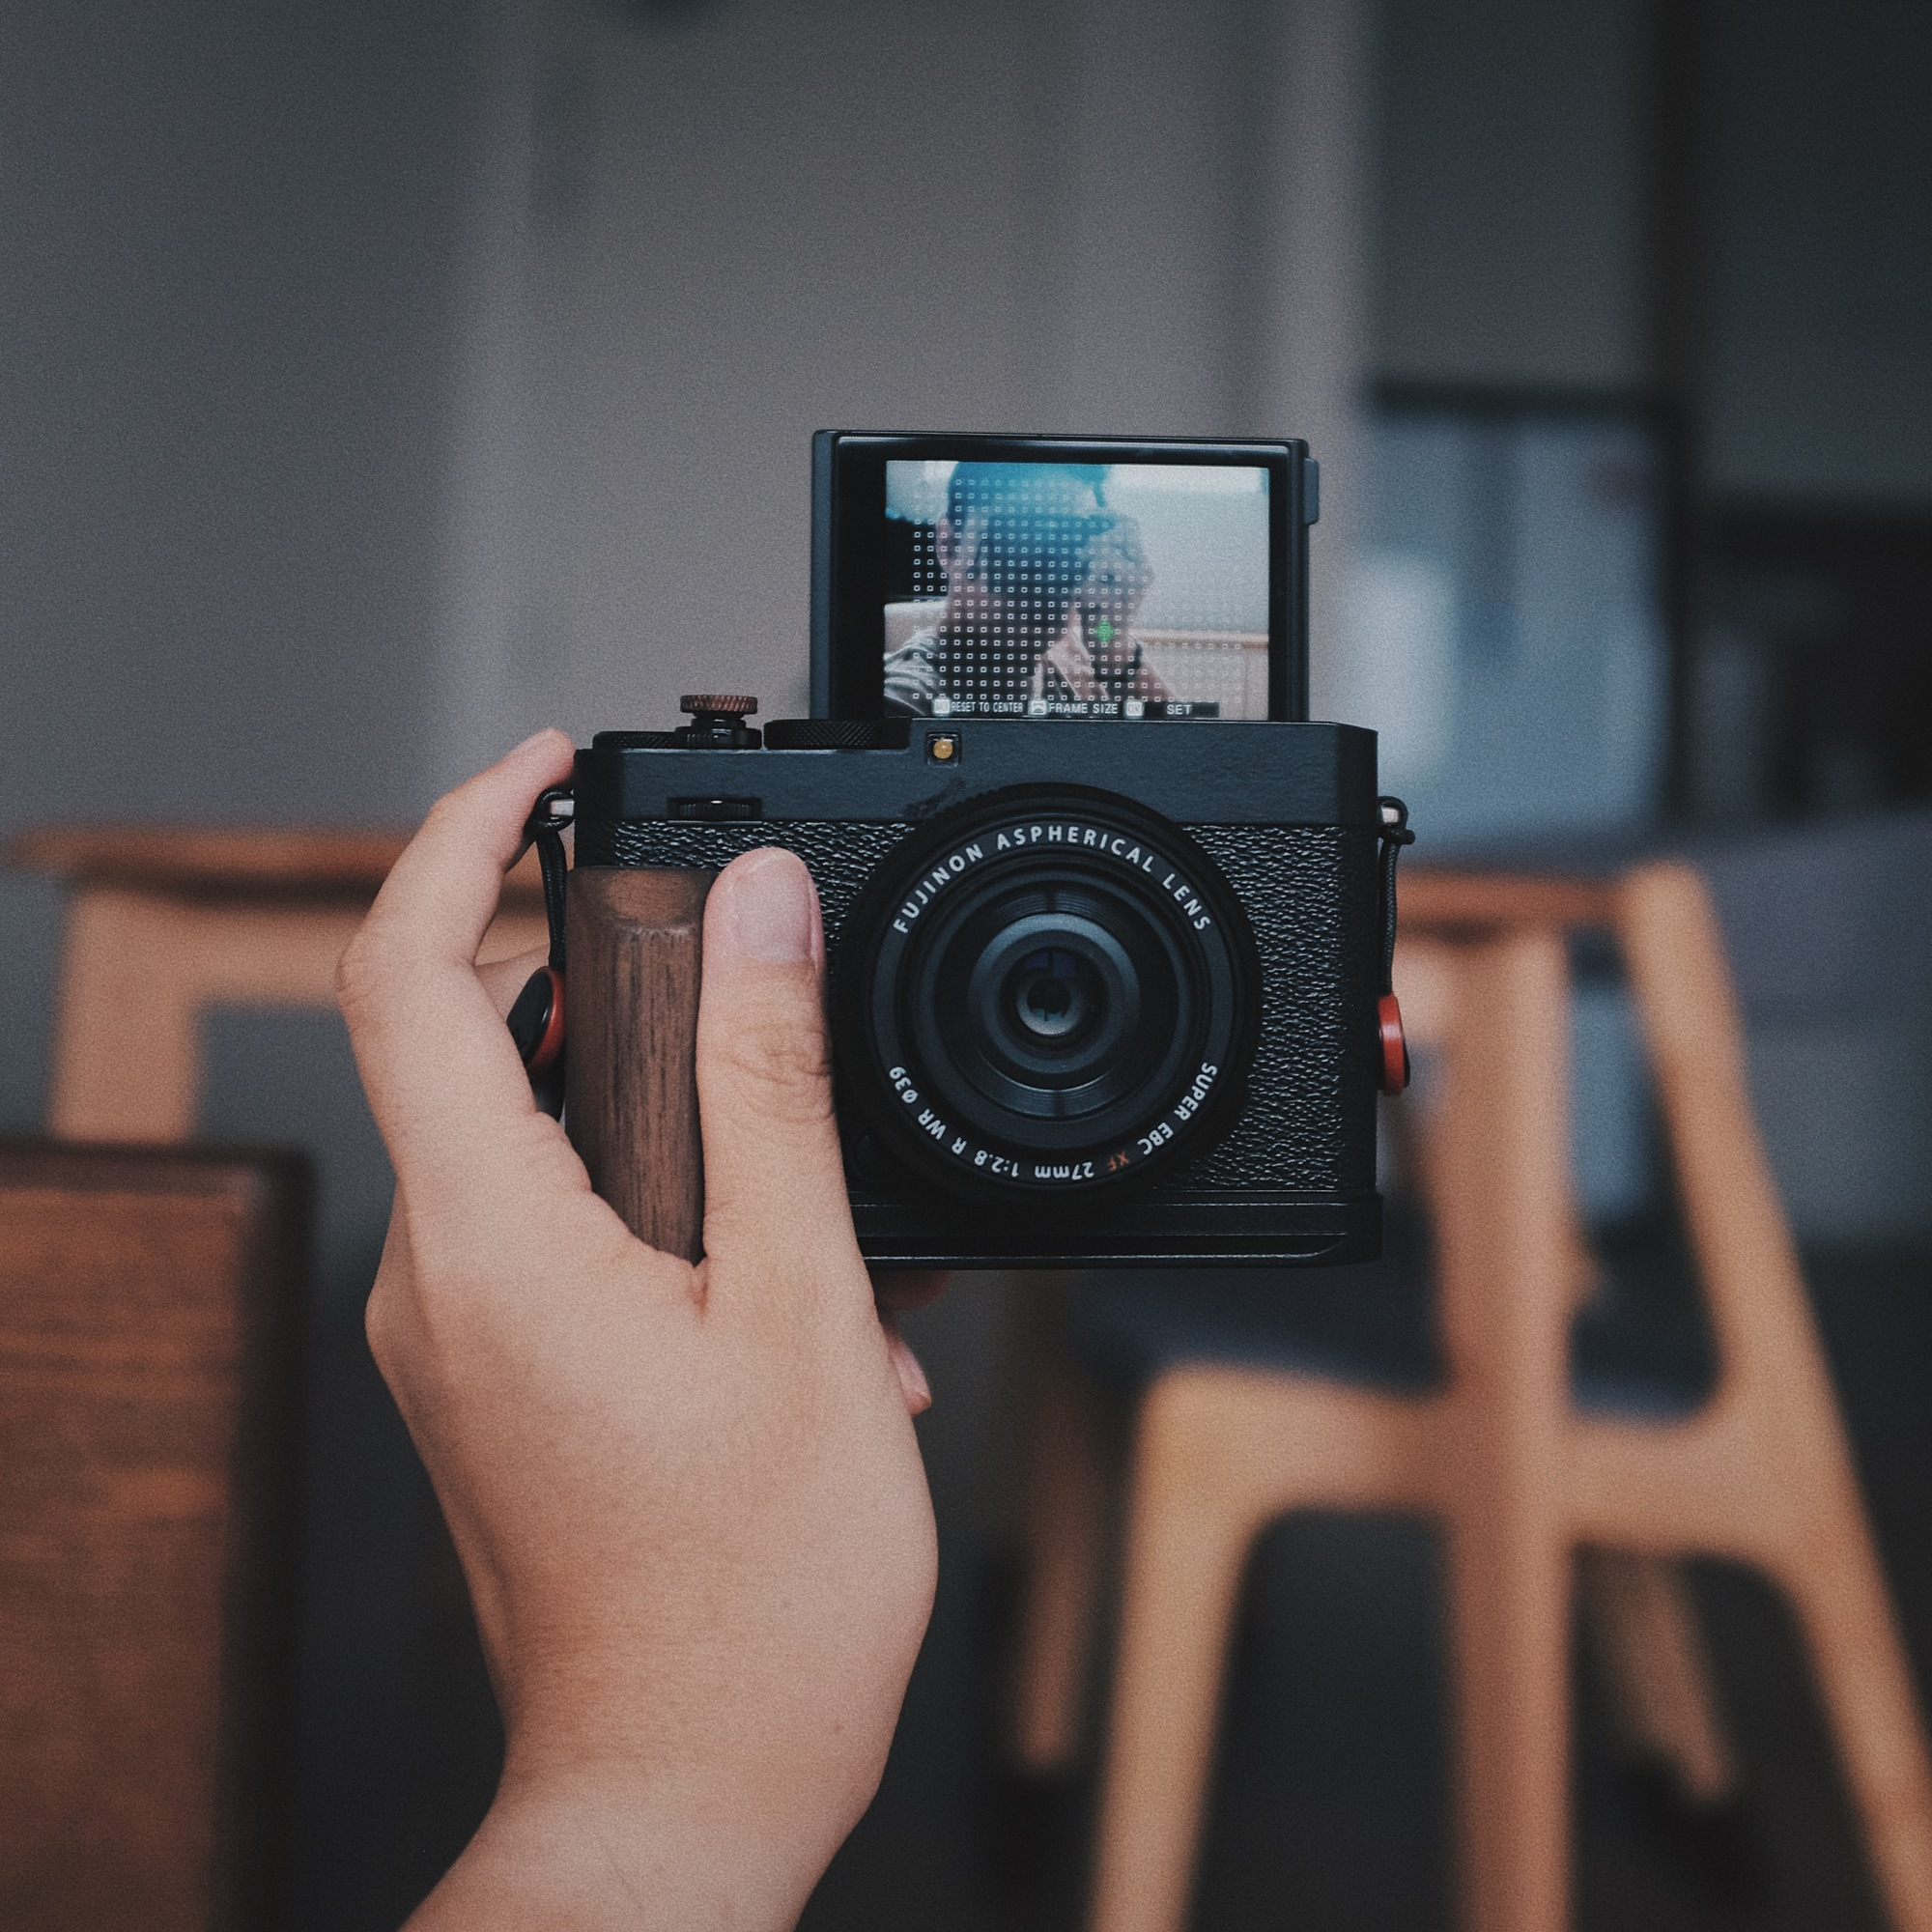
\includegraphics[width=\linewidth]{\envfinaldir/coverpic-prod.jpg}\par
            % \vskip 30pt
            \vfill

            \normalsize\rmfamily\scshape
            \copyright{} The Web Digest Project \hfill\large \envdatestr
        \end{center}
    \end{titlepage}
    % \restoregeometry
}
\newcommand{\simplehref}[1]{%
    \textcolor{blue!80!green}{\href{#1}{#1}}%
}
\renewcommand{\contentsname}{\center\Huge\sffamily\bfseries Contents\par\vskip 20pt}
\newcounter{ipartcounter}
\setcounter{ipartcounter}{0}
\newcommand{\ipart}[1]{
    % \vskip 20pt
    \clearpage
    \stepcounter{ipartcounter}
    \phantomsection
    \addcontentsline{toc}{chapter}{#1}
    % \begin{center}
    %     \Huge
    %     \sffamily\bfseries
    %     #1
    % \end{center}
    % \vskip 20pt plus 7pt
}
\newcounter{ichaptercounter}
\setcounter{ichaptercounter}{0}
\newcommand{\ichapter}[1]{
    % \vskip 20pt
    \clearpage
    \stepcounter{ichaptercounter}
    \phantomsection
    \addcontentsline{toc}{section}{\numberline{\arabic{ichaptercounter}}#1}
    \begin{center}
        \Huge
        \sffamily\bfseries
        #1
    \end{center}
    \vskip 20pt plus 7pt
}
\newcommand{\entrytitlefont}[1]{\subsection*{\raggedright\Large\sffamily\bfseries#1}}
\newcommand{\entryitemGeneric}[2]{
    % argv: title, url
    \parbox{\linewidth}{
        \entrytitlefont{#1}\par\vskip 5pt
        \footnotesize\ttfamily\mdseries
        \simplehref{#2}
    }\vskip 11pt plus 11pt minus 1pt
}
\newcommand{\entryitemGithub}[3]{
    % argv: title, url, desc
    \parbox{\linewidth}{
        \entrytitlefont{#1}\par\vskip 5pt
        \footnotesize\ttfamily\mdseries
        \simplehref{#2}\par\vskip 5pt
        \small\rmfamily\mdseries#3
    }\vskip 11pt plus 11pt minus 1pt
}
\newcommand{\entryitemAp}[3]{
    % argv: title, url, desc
    \parbox{\linewidth}{
        \entrytitlefont{#1}\par\vskip 5pt
        \footnotesize\ttfamily\mdseries
        \simplehref{#2}\par\vskip 5pt
        \small\rmfamily\mdseries#3
    }\vskip 11pt plus 11pt minus 1pt
}
\newcommand{\entryitemHackernews}[3]{
    % argv: title, hnurl, rawurl
    % \parbox{\linewidth}{
    %     \entrytitlefont{#1}\par\vskip 5pt
    %     \footnotesize\ttfamily\mdseries
    %     \simplehref{#3}\par
    %     \textcolor{black!50}{\href{#2}{#2}}
    % }\vskip 11pt plus 11pt minus 1pt
    \begin{minipage}{\linewidth}
            \entrytitlefont{#1}\par\vskip 5pt
            \footnotesize\ttfamily\mdseries
            \simplehref{#3}\par
            \textcolor{black!50}{\href{#2}{#2}}
    \end{minipage}\par\vskip 11pt plus 11pt minus 1pt
}







\begin{document}

\makeheader

\tableofcontents\clearpage




\ipart{Developers}
\ichapter{Hacker News}
\entryitemTwoLinks{Debian 13 "Trixie"}{https://news.ycombinator.com/item?id=44848782}{https://www.debian.org/News/2025/20250809}

\entryitemTwoLinks{A CT scanner reveals surprises inside the 386 processor's ceramic package}{https://news.ycombinator.com/item?id=44848293}{https://www.righto.com/2025/08/intel-386-package-ct-scan.html}

\entryitemTwoLinks{Knuth on ChatGPT (2023)}{https://news.ycombinator.com/item?id=44848259}{https://cs.stanford.edu/~knuth/chatGPT20.txt}

\entryitemTwoLinks{A brief history of the absurdities of the Soviet Union}{https://news.ycombinator.com/item?id=44847481}{https://laurivahtre.ee/empire-of-the-absurd/}

\entryitemTwoLinks{My Lethal Trifecta talk at the Bay Area AI Security Meetup}{https://news.ycombinator.com/item?id=44846922}{https://simonwillison.net/2025/Aug/9/bay-area-ai/}

\entryitemTwoLinks{MCP overlooks hard-won lessons from distributed systems}{https://news.ycombinator.com/item?id=44846871}{https://julsimon.medium.com/why-mcps-disregard-for-40-years-of-rpc-best-practices-will-burn-enterprises-8ef85ce5bc9b}

\entryitemTwoLinks{Mexico to US livestock trade halted due to screwworm spread}{https://news.ycombinator.com/item?id=44846758}{https://www.usda.gov/about-usda/news/press-releases/2025/07/09/secretary-rollins-takes-decisive-action-and-shuts-down-us-southern-border-ports-livestock-trade-due}

\entryitemTwoLinks{The dead need right to delete their data so they can't be AI-ified, lawyer says}{https://news.ycombinator.com/item?id=44846323}{https://www.theregister.com/2025/08/09/dead\_need\_ai\_data\_delete\_right/}

\entryitemTwoLinks{OpenFreeMap survived 100k requests per second}{https://news.ycombinator.com/item?id=44846318}{https://blog.hyperknot.com/p/openfreemap-survived-100000-requests}

\entryitemTwoLinks{Show HN: The current sky at your approximate location, as a CSS gradient}{https://news.ycombinator.com/item?id=44846281}{https://sky.dlazaro.ca}

\entryitemTwoLinks{Long-term exposure to outdoor air pollution linked to increased risk of dementia}{https://news.ycombinator.com/item?id=44846164}{https://www.cam.ac.uk/research/news/long-term-exposure-to-outdoor-air-pollution-linked-to-increased-risk-of-dementia}

\entryitemTwoLinks{Stanford to continue legacy admissions and withdraw from Cal Grants}{https://news.ycombinator.com/item?id=44846130}{https://www.forbes.com/sites/michaeltnietzel/2025/08/08/stanford-to-continue-legacy-admissions-and-withdraw-from-cal-grants/}

\entryitemTwoLinks{Ratfactor's illustrated guide to folding fitted sheets}{https://news.ycombinator.com/item?id=44845839}{https://ratfactor.com/cards/fitted-sheets}

\entryitemTwoLinks{Jan – Ollama alternative with local UI}{https://news.ycombinator.com/item?id=44845272}{https://github.com/menloresearch/jan}

\entryitemTwoLinks{Partially Matching Zig Enums}{https://news.ycombinator.com/item?id=44845017}{https://matklad.github.io/2025/08/08/partially-matching-zig-enums.html}

\entryitemTwoLinks{Sandstorm- self-hostable web productivity suite}{https://news.ycombinator.com/item?id=44844394}{https://sandstorm.org/}

\entryitemTwoLinks{What the Windsurf sale means for the AI coding ecosystem}{https://news.ycombinator.com/item?id=44843801}{https://ethanding.substack.com/p/windsurf-gets-margin-called}

\entryitemTwoLinks{Let's properly analyze an AI article for once}{https://news.ycombinator.com/item?id=44843605}{https://nibblestew.blogspot.com/2025/08/lets-properly-analyze-ai-article-for.html}

\entryitemTwoLinks{Dial-up Internet to be discontinued}{https://news.ycombinator.com/item?id=44843369}{https://help.aol.com/articles/dial-up-internet-to-be-discontinued}

\entryitemTwoLinks{Our European search index goes live}{https://news.ycombinator.com/item?id=44841741}{https://blog.ecosia.org/launching-our-european-search-index/}\ichapter{Phoronix}
\entryitemGeneric{\hskip 0pt{}Btrfs Has Saved Meta "Billions Of Dollars" In Infrastructure Costs}{https://www.phoronix.com/news/Btrfs-Saves-Meta-Billions}

\entryitemGeneric{\hskip 0pt{}Debian 13.0 "Trixie" Now Available - Powered By Linux 6.12 LTS}{https://www.phoronix.com/news/Debian-13.0-Released}

\entryitemGeneric{\hskip 0pt{}Linux 6.17 EFI Stub Will Try To Maintain a Cleaner Boot Experience}{https://www.phoronix.com/news/Linux-6.17-EFI-Stub-Clean-Boot}

\entryitemGeneric{\hskip 0pt{}Vulkan 1.4.325 Released With Untyped Pointers Extension}{https://www.phoronix.com/news/Vulkan-1.4.325-Released}

\entryitemGeneric{\hskip 0pt{}Linus Torvalds Rejects RISC-V Changes For Linux 6.17: "Garbage"}{https://www.phoronix.com/news/Linux-6.17-RISC-V-Rejected}

\entryitemGeneric{\hskip 0pt{}GNU/Hurd Now An Official Platform For SDL Cross-Platform Gaming Library}{https://www.phoronix.com/news/SDL-GNU-Hurd-Platform}

\entryitemGeneric{\hskip 0pt{}GNOME Mutter On Wayland Adds ICC Profile Support, Backlight Improvements}{https://www.phoronix.com/news/GNOME-Mutter-Wayland-ICC}

\entryitemGeneric{\hskip 0pt{}KDE Plasma 6.5 Continues Seeing More Features Added \& Polishing}{https://www.phoronix.com/news/Plasma-6.5-Early-August-2025}

\entryitemGeneric{\hskip 0pt{}Additional Intel Linux Drivers Left Orphaned \& Maintainers Let Go}{https://www.phoronix.com/news/Intel-More-Orphans-Maintainers}


\ipart{Developers~~~~(zh-Hans)}
\ichapter{Solidot}
\entryitemGeneric{\hskip 0pt{}中国主要太阳能公司去年裁员近三分之一}{https://www.solidot.org/story?sid=81994}

\entryitemGeneric{\hskip 0pt{}Windows 10 的 30 美元扩展安全更新支持单一账号 10 台设备}{https://www.solidot.org/story?sid=81993}

\entryitemGeneric{\hskip 0pt{}Linux 桌面市场份额达到 6\%}{https://www.solidot.org/story?sid=81992}

\entryitemGeneric{\hskip 0pt{}OpenAI 发布 GPT-5}{https://www.solidot.org/story?sid=81991}

\entryitemGeneric{\hskip 0pt{}科学家重新创造宇宙第一种分子}{https://www.solidot.org/story?sid=81990}

\entryitemGeneric{\hskip 0pt{}研究显示大模型生成虚假临床信息的可能性高于五成}{https://www.solidot.org/story?sid=81989}

\entryitemGeneric{\hskip 0pt{}特朗普呼吁陈立武立即辞职}{https://www.solidot.org/story?sid=81988}

\entryitemGeneric{\hskip 0pt{}以色列在微软服务器上储存了数百万巴勒斯坦人的电话呼叫}{https://www.solidot.org/story?sid=81987}

\entryitemGeneric{\hskip 0pt{}来自深海细菌的多糖能导致癌细胞自毁}{https://www.solidot.org/story?sid=81986}

\entryitemGeneric{\hskip 0pt{}日本人口连续 16 年减少}{https://www.solidot.org/story?sid=81985}

\entryitemGeneric{\hskip 0pt{}《战地6》和《使命召唤 黑色行动 7》都要求 PC 玩家启用 Secure Boot}{https://www.solidot.org/story?sid=81984}

\entryitemGeneric{\hskip 0pt{}特朗普威胁对芯片征收 100\% 关税,除非在美建厂或承诺建厂}{https://www.solidot.org/story?sid=81983}

\entryitemGeneric{\hskip 0pt{}日本禁止苹果 iOS 限制第三方浏览器引擎}{https://www.solidot.org/story?sid=81982}\ichapter{V2EX}
\entryitemGeneric{\hskip 0pt{}[问与答] 有没有什么送男生的七夕礼物推荐? 3000 元左右的}{https://www.v2ex.com/t/1151308}

\entryitemGeneric{\hskip 0pt{}[宽带症候群] 诡异的断网}{https://www.v2ex.com/t/1151307}

\entryitemGeneric{\hskip 0pt{}[分享发现] 大家看这样刑不刑?}{https://www.v2ex.com/t/1151306}

\entryitemGeneric{\hskip 0pt{}[Solana] 请教下\$v2ex 有白皮书吗?在哪里查看}{https://www.v2ex.com/t/1151304}

\entryitemGeneric{\hskip 0pt{}[macOS] 看起来之前几个版本的 Caps 键按不下去的问题似乎在 Tahoe 版本得到了解决?}{https://www.v2ex.com/t/1151302}

\entryitemGeneric{\hskip 0pt{}[程序员] [开源] 简历筛选助手: 精准识别优秀候选人}{https://www.v2ex.com/t/1151301}

\entryitemGeneric{\hskip 0pt{}[Debian] Debian 13 ``trixie'' released}{https://www.v2ex.com/t/1151300}

\entryitemGeneric{\hskip 0pt{}[微信] 更新了 mac 4.0 版微信,经常自动退出帐号}{https://www.v2ex.com/t/1151299}

\entryitemGeneric{\hskip 0pt{}[汽车] 部分汽车品牌批量召回,看看有没有你的汽车}{https://www.v2ex.com/t/1151298}

\entryitemGeneric{\hskip 0pt{}[酷工作] [京东直招 / 北京] 组内直招前端开发}{https://www.v2ex.com/t/1151297}

\entryitemGeneric{\hskip 0pt{}[程序员] 天天搁这儿吹人工智能,我就不信你们能把这张图做出``王境泽嚣张指人''效果}{https://www.v2ex.com/t/1151295}

\entryitemGeneric{\hskip 0pt{}[程序员] 现在还有什么提示词小技巧吗}{https://www.v2ex.com/t/1151294}

\entryitemGeneric{\hskip 0pt{}[iPhone] iPhone 的第三方 app 有时候开摄像头扫码结果一片黑,但是相机可以正常打开}{https://www.v2ex.com/t/1151293}

\entryitemGeneric{\hskip 0pt{}[Solana] \$v2ex 股东速成版}{https://www.v2ex.com/t/1151292}

\entryitemGeneric{\hskip 0pt{}[推广] 一个不需要注册、不插广告的小工具,帮你把照片一键变成可爱风格图片。技术栈是 Next.js + Cloudflare Pages Functions + R2 + KV,纯前端页面 + 边缘函数,访问速度还不错。}{https://www.v2ex.com/t/1151290}

\entryitemGeneric{\hskip 0pt{}[移民] awesome-run 中国打工人的润学指南}{https://www.v2ex.com/t/1151289}

\entryitemGeneric{\hskip 0pt{}[推广] SeekCode 第二弹:对接 AI 的新能力}{https://www.v2ex.com/t/1151287}

\entryitemGeneric{\hskip 0pt{}[反馈] 连接到 Solana 是否可以提供输入地址的选项?}{https://www.v2ex.com/t/1151285}

\entryitemGeneric{\hskip 0pt{}[Google] Pixel 的 谷歌账号被登出 要求使用 GV 自证身份 鸡与蛋的哲学?}{https://www.v2ex.com/t/1151284}

\entryitemGeneric{\hskip 0pt{}[问与答] Emby 动态海报墙问题}{https://www.v2ex.com/t/1151283}

\entryitemGeneric{\hskip 0pt{}[智能家电] 202508 的 TCP/雷鸟电视还能接入 HA 吗、}{https://www.v2ex.com/t/1151282}

\entryitemGeneric{\hskip 0pt{}[问与答] 那么这个 Windows 右下角弹窗的两个按钮到底分别干什么?}{https://www.v2ex.com/t/1151281}

\entryitemGeneric{\hskip 0pt{}[Chrome] chrome 的 DOH 是摆设吧?}{https://www.v2ex.com/t/1151280}

\entryitemGeneric{\hskip 0pt{}[分享发现] [开源][跨平台]超级无敌爆炸好用的截图软件!一键 OCR、录屏、翻译、AI 对话,火热开发中🔥}{https://www.v2ex.com/t/1151279}

\entryitemGeneric{\hskip 0pt{}[YouTube] 尝试做油管,几乎没播放,好难}{https://www.v2ex.com/t/1151278}

\entryitemGeneric{\hskip 0pt{}[移民] 一年半拿到日本永驻分享下经验}{https://www.v2ex.com/t/1151276}

\entryitemGeneric{\hskip 0pt{}[问与答] 怎样禁止 Windows 的这种 "预测触摸轨迹" 的行为?}{https://www.v2ex.com/t/1151275}

\entryitemGeneric{\hskip 0pt{}[Solana] What does Livid want?}{https://www.v2ex.com/t/1151274}

\entryitemGeneric{\hskip 0pt{}[Apple] macOS 发消息居然可以是短信?}{https://www.v2ex.com/t/1151273}

\entryitemGeneric{\hskip 0pt{}[程序员] claude 封号的核心原因:一张完整的``红线''清单}{https://www.v2ex.com/t/1151272}

\entryitemGeneric{\hskip 0pt{}[五笔字型输入法] 安卓同文输入法的 14 键五笔好像终于能用了}{https://www.v2ex.com/t/1151271}

\entryitemGeneric{\hskip 0pt{}[Google] Google 账户风控新政策,需要原手机号发短信!发短信!}{https://www.v2ex.com/t/1151269}

\entryitemGeneric{\hskip 0pt{}[问与答] 如何远程控制安卓手机}{https://www.v2ex.com/t/1151268}

\entryitemGeneric{\hskip 0pt{}[微信] 话说微信小程序到底支持 wasm 吗?文档说支持,但我用 Claude Code 写,老是报错}{https://www.v2ex.com/t/1151266}

\entryitemGeneric{\hskip 0pt{}[摄影] 现在还适合买 A7R5 么?廉颇老矣,尚能饭否?}{https://www.v2ex.com/t/1151265}

\entryitemGeneric{\hskip 0pt{}[生活] 北京五环放开限购了, 上海外环放开限购 也不远了吧.}{https://www.v2ex.com/t/1151264}

\entryitemGeneric{\hskip 0pt{}[问与答] switch 萌新买了 switch2,港版的,有一些问题想求教各位大佬}{https://www.v2ex.com/t/1151263}

\entryitemGeneric{\hskip 0pt{}[酷工作] 帮朋友招一个高级研发工程师, Python /Go 背景,懂云原生/虚拟化的开发}{https://www.v2ex.com/t/1151261}

\entryitemGeneric{\hskip 0pt{}[分享创造] 独立开发前线周刊第 8 期:寻找更多的失败}{https://www.v2ex.com/t/1151260}

\entryitemGeneric{\hskip 0pt{}[酷工作] 招聘(远程办公-web3) Golang 工程师 测试工程师 前端工程师(Nodejs / React) Flutter(app) DevOps 工程师 大数据开发工程师 Product Manager}{https://www.v2ex.com/t/1151259}

\entryitemGeneric{\hskip 0pt{}[职场话题] 哪个多签钱包安全性好并可以使用波场链}{https://www.v2ex.com/t/1151256}

\entryitemGeneric{\hskip 0pt{}[问与答] 2C4G 服务器建议安装哪个 Windows server 版本?}{https://www.v2ex.com/t/1151255}

\entryitemGeneric{\hskip 0pt{}[Web3] 我准备写一个关于 web3 的科普,主题就叫「信任有多少成本」,讲一下在现实生活中,因信任造成了多少成本,而 web3 是否会降低以及会降低多少成本}{https://www.v2ex.com/t/1151252}

\entryitemGeneric{\hskip 0pt{}[问与答] 2025 年快过完了,不上班在家里做的可以养活自己的兼职推荐??}{https://www.v2ex.com/t/1151250}

\entryitemGeneric{\hskip 0pt{}[问与答] 用了十年的 iPhone ,想换一款没有限制的安卓,大家懂的,应该买哪个品牌的。}{https://www.v2ex.com/t/1151249}

\entryitemGeneric{\hskip 0pt{}[分享创造] [网站自荐] 体检参考助手 - 智能体检参考与知识整理平台,按年龄/性别快速生成体检前参考清单。涵盖基础/专科/重点/可选四类项目,配套注意事项与流程参考,信息结构化、可打印、可收藏,帮助你高效做好体检前功课(仅供参考,需医生确认)。}{https://www.v2ex.com/t/1151248}

\entryitemGeneric{\hskip 0pt{}[Kubernetes] 有人用过 victoria metrics stack 吗?}{https://www.v2ex.com/t/1151247}

\entryitemGeneric{\hskip 0pt{}[问与答] 有没有 pc 端质量高一些的开车游戏}{https://www.v2ex.com/t/1151246}

\entryitemGeneric{\hskip 0pt{}[酷工作] 🚀 招募 Web3 前端工程师}{https://www.v2ex.com/t/1151245}

\entryitemGeneric{\hskip 0pt{}[Podcast] [神器分享] 终于找到了解决英文播客痛点的工具,英文播客变自然人声的中文,还能双语对照学英语 - NativePod}{https://www.v2ex.com/t/1151243}


\ipart{Generic News}







\clearpage
\leavevmode\vfill
\footnotesize

Copyright \copyright{} 2023-2025 Neruthes and other contributors.

This document is published with CC BY-NC-ND 4.0 license.

The entries listed in this newsletter may be copyrighted by their respective creators.

This newsletter is generated by the Web Digest project.

The newsletters are also delivered via Telegram channel \CJKunderline{\href{https://t.me/webdigestchannel}{https://t.me/webdigestchannel}}.\\
RSS feed is available at \CJKunderline{\href{https://webdigest.pages.dev/rss.xml}{https://webdigest.pages.dev/rss.xml}}.

This newsletter is available in PDF at
\CJKunderline{\href{https://webdigest.pages.dev/}{https://webdigest.pages.dev/}}.

The source code being used to generate this newsletter is available at\\
\CJKunderline{\href{https://github.com/neruthes/webdigest}{https://github.com/neruthes/webdigest}}.

This newsletter is also available in
\CJKunderline{\href{http://webdigest.pages.dev/readhtml/\envyear/WebDigest-20250810.html}{HTML}} and
\CJKunderline{\href{https://github.com/neruthes/webdigest/blob/master/markdown/\envyear/WebDigest-20250810.md}{Markdown}}.


\coverpic{https://unsplash.com/photos/a-blurry-picture-of-a-yellow-and-blue-object-KDCd2VmZYGs}{Sindy Süßengut}


\end{document}
